\begin{tikzpicture}[x=0.75cm,y=-0.75cm,step=0.75cm]
	\usetikzlibrary{decorations.pathreplacing, arrows.meta}
	%\draw [help lines] (0,0) grid (27,30);

	% Header
	\draw[thick] (2,1) -- (8,1);
	\node[anchor=south east] at (2,1) {Date:};
	\draw[thick] (12,1) -- (16,1);
	\node[anchor=south east] at (12,1) {Common Time:};
	\draw[thick] (18,1) -- (27,1);
	\node[anchor=south east] at (18,1) {Body:};

	% Table 1
	\draw[dotted, thick]	(2,3) -- (7,3); \draw[dotted, thick] 	(9,3) -- (14,3);
	\draw[thick] 		(2,4) -- (7,4);	\draw[thick] 		(9,4) -- (14,4);
	\draw[dotted, thick]	(2,5) -- (7,5);	\draw[dotted, thick] 	(9,5) -- (14,5);
	\draw[thick] 		(2,6) -- (7,6);	\draw[thick] 		(9,6) -- (14,6);
	\draw[double, thick]	(7,2) -- (7,5);	\draw[double, thick]	(14,2) -- (14,5);
	\draw[dotted, thick]	(2,7) -- (14,7);
	\draw[thick]		(2,8) -- (14,8);
	\draw[dotted, thick]	(2,9) -- (14,9);
	\node at (1,2.5) { % Sun/star limb diagram
		\begin{tikzpicture}
			\usetikzlibrary{shapes.geometric}
			\draw[thick] (0.5,0) -- (1.5,0);
			\node[circle, fill=black, draw] at (1,0.25) {};
			\draw[thick] (0,1) -- (1.5,1);
			\node[circle, fill=black, draw] at (0.25,0.75) {};
			\node[star, star points=6, star point ratio=3, inner sep=1.25, fill=black, draw] at (1,1) {};
		\end{tikzpicture} };
	\node at (8,2.375) { % Lunar limb diagram
		\pgfmathsetmacro{\r}{0.25} % radius
		\pgfmathsetmacro{\a}{135} % rotation
		\begin{tikzpicture}
			\usetikzlibrary{shapes.geometric}
			\draw (0.5,0) -- (1.5,0);
			\draw (0,1) -- (1,1);
			\draw let \n1 = {veclen(\r, \r)},
				\n2 = {\r*(sin(\a-90))}, % from cycloid formulas
				\n3 = {\r*(1-cos(\a-90))} in 
				(0.5+\n2,1-\n3) arc (180-\a:360-\a:0.25) arc (-45-\a:-135-\a:\n1);
			\draw let \n1 = {veclen(\r, \r)},
				\n2 = {\r*(sin(\a-90))},
				\n3 = {\r*(1-cos(\a-90))} in 
				(1-\n2,\n3) arc (0-\a:180-\a:0.25) arc (135-\a:45-\a:\n1);
		\end{tikzpicture} };
	\node[anchor=south east] at (2,4) {Table \large 1};
	\node[anchor=south east] at (2,5) {\large Sa};
	\node[anchor=south east, align=center, scale=0.8] at (2,6) {(subtract \\ lesser)};
	\node[anchor=south east] at (2,7) {\large Ma$\sim$Sa};
	\node[anchor=south east] at (2,9) {\large H$\sim$H};
	\node[anchor=south east] at (9,4) {Table \large 1};
	\node[anchor=south east] at (9,5) {\large Ma};
	\node at (8,5.6) { % crossed arrows
		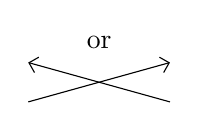
\begin{tikzpicture}
			\draw[-{Straight Barb[scale=1.25]}] (0,0) -- (1.8,0.5);
			\draw[-{Straight Barb[scale=1.25]}] (1.8,0) -- (0,0.5);
			\node at (0.9,0.75) {or};
		\end{tikzpicture} };

	% Table 2-3
	\draw[thick]		(20,3) -- (23,3) node [midway, below] {Moon};
	\draw[thick]		(24,3) -- (27,3) node [midway, below] {Venus/Mars};
	\draw[dotted, thick]	(18,5) -- (22,5); \draw[dotted, thick] 	(23,5) -- (27,5);
	\draw[dotted, thick]	(18,6) -- (22,6); \draw[dotted, thick] 	(23,6) -- (27,6);
	\draw[thick]		(18,7) -- (22,7); \draw[thick] 		(23,7) -- (27,7);
	\draw[dotted, thick]	(18,8) -- (22,8); \draw[dotted, thick] 	(23,8) -- (27,8);
	\node[anchor=south east] at (20,3) {HP:};
	\draw[decorate, decoration = {brace}] (17.8,5.8) -- (17.8,4.2) node [name=tab2, midway, left] {Table \large 2\;};
	\node[anchor=south east] at (18,7) {Table \large 3};
	\node[anchor=north] at (25,8) {\large Q};
	\draw (23,7) -- (23,8); \draw (27,7) -- (27,8); \draw (27,8) arc[start angle=0, end angle=180, x radius=2, y radius=1];
	\draw[-{Straight Barb[scale=1.25]},thick] (18,7.5) -- (15,7.5) node [midway, below] {(round)};

	% Table 4-6
	\draw[dotted, thick]	(18,11) -- (22,11);
	\draw[thick]		(18,12) -- (22,12);
	\draw[dotted, thick]	(18,13) -- (22,13);
	\draw[thick]		(18,14) -- (22,14);
	\draw[dotted, thick]	(18,15) -- (22,15);
	\node[anchor=south east] at (18,11) {Table \large 4};
	\node[anchor=south east] at (18,12) {Sun? \;\large 5};
	\node[anchor=south east, align=left] at (18,14) {Low Sun \\ or Moon? \;\large 6};
	\draw[decorate, decoration = {brace}] (22.2,10.2) -- (22.2,11.8) node [midway, right] {\;add};
	\draw[-{Straight Barb[scale=1.25]},thick] (18,14.5) -- (12,14.5) node [midway, below] {(round)};

	% Sextant distance table
	\draw[dotted,thick]	(5,12) -- (11,12);
	\draw[thick]		(5,13) -- (11,13);
	\draw[dotted,thick]	(5,14) -- (11,14);
	\draw[thick]		(5,15) -- (11,15);
	\draw[dotted,thick]	(5,16) -- (11,16);
	\draw[thick]		(5,17) -- (11,17);
	\draw[dotted,thick]	(5,18) -- (11,18);
	\draw[dotted,thick]	(5,19) -- (11,19);
	\node[anchor=east] at (1.5,11.5) {\large \textbf{Ds}};
	\draw[-{Straight Barb[scale=1.25]},thick] (1.5,11.5) -- (4.75,11.5) node [midway, above, scale=0.8] {Sextant Distance\;};
	\node[anchor=south east] at (5,13) {Index error};
	\draw[decorate, decoration = {brace}] (4.5,14) -- (4.5,15) node [midway, left, align=right] {Near Limb: $+$ \\ Far Limb: $-$};
	\node[anchor=south east] at (5,16) {\large Da};
	\node[anchor=south east] at (5,17) {\large Ma$\sim$Sa};
	\node[anchor=south east] at (5,18) {\large Da$-($Ma$\sim$Sa$)$};
	\node[anchor=south east] at (5,19) {\large Da$+($Ma$\sim$Sa$)$};
	\draw[-{Straight Barb[scale=1.25]},thick,dashed] (11,17.5) -- (17,17.5);
	\draw[-{Straight Barb[scale=1.25]},thick,dashed] (11,18.5) -- (17,18.5);

	% K table
	\draw[dashed,thick]	(21,17) -- (21,25);
	\draw[dotted,thick]	(18,18) -- (24,18);
	\draw[thick]		(18,19) -- (24,19);
	\draw[thick]		(18,20) -- (24,20);
	\draw[dotted,thick]	(18,21) -- (25,21);
	\draw[thick]		(18,22) -- (25,22);
	\draw[dotted,thick]	(18,23) -- (24,23);
	\draw[thick]		(18,24) -- (24,24);
	\draw[dotted,thick]	(18,25) -- (24,25);
	\node[anchor=south east] at (18,18) {\large K};
	\node[anchor=south east] at (18,19) {\large K};
	\draw[decorate, decoration = {brace}] (24.2,17.2) -- (24.2,18.8) node [midway, right] {\;add};
	\draw[decorate, decoration = {brace}] (25.2,20.2) -- (25.2,21.8) node [midway, right] {\;add};
	\draw[-{Straight Barb[scale=1.25]}] (17.9,19.5) arc (270:180:0.8) node [below] {half};
	\node[anchor=south east] at (18,22) {\large Q};
	\node [anchor=south west] at (24,23) {(round)};
	\node[anchor=south west, align=center, scale=0.8] at (24,24) {(subtract \\ lesser)};
	\node at (17,23.6) { % crossed arrows
		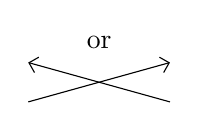
\begin{tikzpicture}
			\draw[-{Straight Barb[scale=1.25]}] (0,0) -- (1.8,0.5);
			\draw[-{Straight Barb[scale=1.25]}] (1.8,0) -- (0,0.5);
			\node at (0.9,0.75) {or};
		\end{tikzpicture} };
	\node at (17,24.6) { % gaussian crossed arrows
		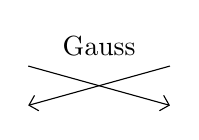
\begin{tikzpicture}
			\draw[{Straight Barb[scale=1.25]}-] (0,0) -- (1.8,0.5);
			\draw[{Straight Barb[scale=1.25]}-] (1.8,0) -- (0,0.5);
			\node at (0.9,0.75) {Gauss};
		\end{tikzpicture} };

	% Gaussians table
	\draw[dashed,thick]	(13,22) -- (13,25);
	\draw[dotted,thick]	(10,23) -- (16,23);
	\draw[thick]		(10,24) -- (16,24);
	\draw[dotted,thick]	(10,25) -- (16,25);
	\draw[double,thick]	(2,25) -- (8,25);
	\node[anchor=south east, name=hh] at (8,23) {\large H$\sim$H};
	\node[anchor=south east, name=k] at (10,23) {\large K};
	\draw[-{Straight Barb[scale=1.25]},thick,dashed] (hh) -- (k);
	\node[anchor=south east] at (2,25) {\large D};
	\node[anchor=south] at (9,25) {\large \reflectbox{K}};



	\foreach \position in {(4,3), (11,3), (5,25), (8,12)} { % degree, minute markers with tick
		\draw[anchor=south] \position node{\LARGE$^\circ$};
		\draw[anchor=south] \position+(2,0) node{\LARGE$\overset{'}{.}$}; }
	\foreach \position in {(4,5), (4,6), (4,7), (4,9), (11,5), (11,6), (11,7), (11,9), (8,14), % degree, minute markers without tick
			       (8,16), (8,17), (8,18), (8,19)} {
		\draw[anchor=south] \position node{\LARGE$^\circ$};
		\draw[anchor=south] \position+(2,0) node{\LARGE$.$}; }
	\foreach \position in {(6,4), (6,8), (13,4), (13,8), (20,6), (20,7), (20,8), % period
			       (20,12), (20,13), (20,14), (20,15), (10,15), (19,18),
			       (19,19), (19,20), (19,21), (19,23), (19,24), (19,25), (11,23),
			       (11,24), (11,25), (10,13)} {
		\draw[anchor=south] \position node{\LARGE$.$}; }
	\foreach \position in {(22,3), (26,3), (20,5), (20,11)} { % period with tick
		\draw[anchor=south] \position node{\LARGE$\overset{'}{.}$}; }
	\foreach \position in {(26,5), (26,6), (26,7), (26,8), (24,21), (24,22)} { % comma
		\draw[anchor=south] \position node{\LARGE$,$}; }
	\foreach \position in {(4,8), (20,14)} { % minus
		\draw[anchor=south east] \position node{\LARGE$-$}; }
	\foreach \position in {(11,8)} { % plus
		\draw[anchor=south east] \position node{\LARGE$+$}; }
\end{tikzpicture}
